\documentclass[14pt, a4paper]{extreport}

\usepackage{geometry}

\usepackage{graphicx}
\graphicspath{{./Images/}}

\usepackage{fontspec}
\usepackage{polyglossia}
\usepackage{hyphenat}

\setotherlanguage{english}

\defaultfontfeatures{Ligatures=TeX}

\setmainfont{Times New Roman}
\setsansfont{Arial}
\setmonofont[Scale=0.8]{DejaVu Sans Mono}

\usepackage{unicode-math}
\setmathfont{Latin Modern Math}

\geometry{
	a4paper,
	left=25mm,
	right=10mm,
	top=15mm,
	bottom=15mm,
}

\usepackage{setspace}
\onehalfspacing

\usepackage{caption}
\usepackage{float}
\usepackage{listings, listings-rust}
\usepackage{xcolor}

\definecolor{codegreen}{rgb}{0,0.6,0}
\definecolor{codegray}{rgb}{0.5,0.5,0.5}
\definecolor{codepurple}{rgb}{0.58,0,0.82}
\definecolor{backcolour}{rgb}{ 0.976, 0.976, 0.976 }

\usepackage{fancyhdr}
\usepackage{hyperref}
\hypersetup{unicode=true, colorlinks=true, linkcolor=black, urlcolor=black}

\pagestyle{fancy}
\fancyhf{}
\renewcommand\headrulewidth{0pt}
\cfoot{\thepage}

\setlength{\headheight}{18pt}

\usepackage{indentfirst}

% Const
\newcommand{\CourseTitle}{Програмне забезпечення комп'ютерних систем}
\newcommand{\Variant}{5}
\newcommand{\StudentGroup}{ІМ-51мн}
\newcommand{\CourseNumber}{1}
\newcommand{\StudentName}{Ковальов Олександр}
\newcommand{\Teacher}{к.т.н., Русанова Ольга Веніаминівна}
\newcommand{\Year}{2025}

% Change this
\newcommand{\LabNumber}{1}
\newcommand{\Topic}{Лексичний та синтаксичний аналіз}
\newcommand{\SubmissionDate}{14.10.2025}

\lstdefinestyle{mystyle}{
	backgroundcolor=\color{backcolour},   
	commentstyle=\color{codegreen},
	keywordstyle=\color{magenta},
	numberstyle=\tiny\color{codegray},
	stringstyle=\color{codepurple},
	basicstyle=\ttfamily\footnotesize,
	breakatwhitespace=false,         
	breaklines=true,                 
	captionpos=b,                    
	keepspaces=true,                 
	numbers=left,                    
	numbersep=5pt,                  
	showspaces=false,                
	showstringspaces=false,
	showtabs=false,                  
	tabsize=2
}

\lstset{style=mystyle}

\usepackage{enumitem}
\setlist[enumerate]{
	itemsep=0.0\baselineskip,
	left=1.25cm,
	rightmargin=10mm,
	labelsep=0.5cm,
	listparindent=1.25cm,
	parsep=0pt
}

\begin{document}
	\tolerance=350 % Or just increase the number
	\emergencystretch=3em
	
	\begin{titlepage}
		\begin{center}
			{Національний технічний університет України\\
				«Київський політехнічний інститут імені Ігоря Сікорського» \\[1.0em] }
			{Факультет інформатики та обчислювальної техніки\\}
			{Кафедра обчислювальної техніки \\[5.0em]}
			
			{\textbf{ЗВІТ}\\[1em]}
			{\textbf{з лабораторної роботи №\LabNumber} \\}
			{\textbf{з дисципліни "\CourseTitle"} \\[2.0em]}
			
			{\textbf{Тема: \Topic} \\[2.0em]}
			
			{\textbf{Варіант №\Variant} \\[5.0em]}
			
			\begin{flushright}
				Виконав: \\
				Студент \CourseNumber{} курсу, групи \StudentGroup \\
				\StudentName \\[2.0em]
			\end{flushright}
			
			\begin{flushright}
				Перевірила: \\
				\Teacher \\[2.0em]
			\end{flushright}
			
			\begin{flushright}
				Дата здачі: \SubmissionDate \\[5.0em]
			\end{flushright}
		
			\vfill
			КИЇВ -- \Year
		\end{center}
	\end{titlepage}
	
	\setlength{\parindent}{1.25cm}
	
	\textbf{Мета роботи:} навчитися виконувати лексичний та синтаксичний аналіз заданого арифметичного виразу.
	
	\textbf{Вхідні дані:} арифметичний вираз з дужками або в бездужковому записі, елементами якого є константи, імена змінних, алгебраїчні операції та математичні функції.
	
	\textbf{Завдання:} реалізувати лексичний та синтаксичний аналізатор арифметичного виразу з використанням будь-якої мови програмування. Необхідно, щоб аналізатор перевіряв такі типи помилок:
	\begin{enumerate}[noitemsep, nolistsep]
		\item Помилки на початку арифметичного виразу (наприклад, вираз не може починатись із закритої дужки, алгебраїчних операцій * та /);
		\item Помилки, пов’язані з неправильним написанням імен змінних, констант та при необхідності функцій;
		\item Помилки у кінці виразу (наприклад, вираз не може закінчуватись будь-якою алгебраїчною операцією);
		\item Помилки в середині виразу (подвійні операції, відсутність операцій перед або між дужками, операції * або / після відкритої дужки тощо);
		\item Помилки, пов’язані з використанням дужок (нерівна кількість відкритих та закритих дужок, неправильний порядок дужок, пусті дужки).
	\end{enumerate}
	
	Синтаксичний аналізатор потрібно реалізувати за допомогою кінцевого автомату. Результатом виконання даної лабораторної роботи є список помилок, виявлених під час синтаксичного аналізу.
	
	\begin{center}
		\textbf{Хід роботи.}
	\end{center}
	
	В ході лабораторної роботи був написаний застосунок мовою програмування Rust. Він складається з декількох частин -- візуальна частина (фронтенд), яка надає консольний інтерфейс користувачу. Обчислення відбуваються на частині, яка відповідає за логіку (бекенд). Вона поділяється на модулі, які відповідають за лексичний (токенізація) та синтаксичний аналіз.
	
	\begin{figure}[H]
		\centering
		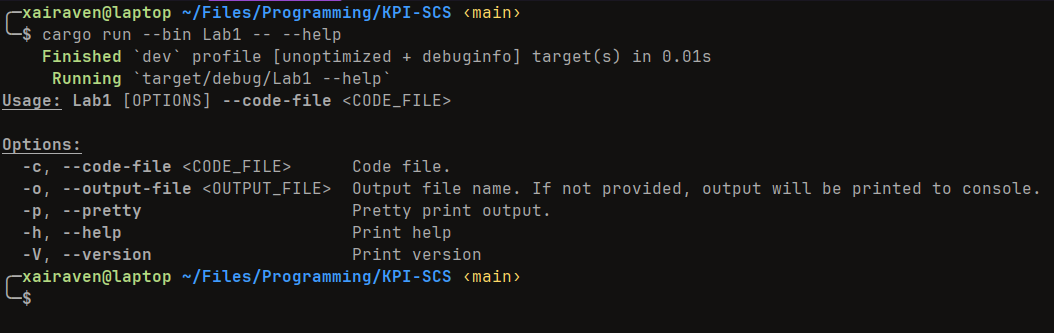
\includegraphics[height=4cm]{1} 
	\end{figure}
	
	Лексичний аналіз (токенізація) потрібен для формалізації вхідного потоку даних. Тобто, кожну логічну частинку тексту можна виділити для того, щоб мати змогу в подальшому їх застосовувати набагато ефективніше, особливо враховуючи систему типів обраної мови програмування. За допомогою типу даних "enum" та додаткової логіки можна повністю класифікувати весь код.
	
	Були виділені основні типи токенів: ідентифікатор, число, знаки плюс, мінус, зірочка, слеш, відсоток, круглі дужки, квадратні дужки, знак оклику, амперсанд, пряма лінія, крапка, кома, лапки, пробіл, таб, нова лінія, та насамкінець невідомий тип токену.
	
	Токен типу "Ідентифікатор" включає в себе всі послідовні символи, якщо вони починаються з букви та містять в собі цифри та нижнє підчеркування. Числа складаються з цифр від 0 до 9. Пробіл містить в собі всі послідовні пробіли. Всі інші типи токенів складаються з відповідних та інтуїтивних символів, по одному на токен.
	
	Сама структура "Токен" складається з трьох полів: тип, позиція в тексті (діапазон) та опціональне значення (потрібне для тексту, чисел, невідомих символів).
	
	Синтаксичний аналіз більш складний. Базова реалізація полягає в абстракції кінечного автомата. По-перше, для аналізу потрібен контекст - ним виступає окрема стуктура, яка містить вектор токенів, поточний індекс (для ітерації по токенам), структура "Статус" (для зберігання стану в логічних змінних), вектор синтаксичних помилок, та стеки круглих, квадратних дужок і лапок.
	
	Типів синтаксичних помилок всього 20: "порожні квадратні дужки", "порожні круглі дужки", "некоректний бінарний літерал", "некоректний шістнадцятковий літерал", неправильне число з плаваючою комою, неправильна назва функції, некоректна назва змінної, неочікувані квадратні дужки, коми, крапки, кінець виразу, нова лінія, операнд, оператор, круглі дужки. Окремо є помилки "невідомий токен", непарні квадратні дужки, круглі дужки, лапки.
	
	Структура "Статус" має три поля: "очікуємо операнд", "очікуємо оператор", та "знаходимося в рядку".
	
	На початку аналізу встановлюється статус "Очікуємо операнд". Далі, з вектору токенів видаляються всі пробіли та таби, які не належать певному рядку.
	
	Після попередньої підготовки вхідного потоку (видалення непотрібних пробілів та табуляцій поза рядковими літералами) виконується поетапний лінійний прохід по вектору токенів. На кожному кроці кінцевий автомат розглядає поточний токен та контекст (поля структури Status, стеки для дужок і лапок, попередні та наступні токени) і приймає одне з наступних рішень:
	
	\begin{enumerate}[noitemsep, nolistsep]
		\item Зрушити індекс на один (типовий випадок для одиничних токенів: оператори, роздільники, прості літерали);
		\item Зрушити індекс на кілька позицій (складні літерали: число-точка-число для чисел з плаваючою крапкою, або префіксні системи числення, які токенізуються як два токени — наприклад \texttt{0} та \texttt{xFF});
		\item Записати синтаксичну помилку в масив errors з вказанням токена та типу помилки;
		\item Змінити внутрішній стан автомата (очікуємо операнд / очікуємо оператор / всередині рядка) та оновити стеки дужок/лапок.
	\end{enumerate}
	
	\bigskip
	
	\textbf{Тестування і приклади результатів.} Для перевірки коректності реалізації створено набір автоматичних юніт-тестів (функції з префіксом \texttt{test\_syntax\_*}), які моделюють різні види помилок: початкові помилки (наприклад, вираз починається з оператора), подвійні оператори, невірні імена змінних та функцій, неправильні числові форми, незбалансовані дужки та незакриті лапки. Загалом реалізовано 18 тестів, що охоплюють як прості, так і складні синтаксичні конструкції.
	
	\begin{figure}[H]
		\centering
		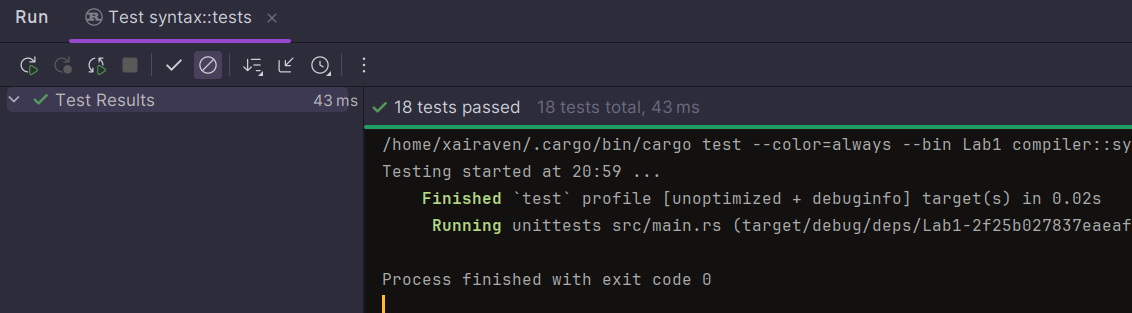
\includegraphics[height=5cm]{2} 
	\end{figure}
	
	Запуск тестів у середовищі розробки Rust виконується стандартною командою:
	\begin{lstlisting}
		cargo test --package Lab1 --bin Lab1
	\end{lstlisting}
	
	\pagebreak
	
	Приклад виводу помилок для виразу
	\texttt{"-a ++ b - 2v*func((t+2 -, sin(x/*2.01.2), )/8(-)**"} (перший юніт-тест):
	\begin{lstlisting}
		-a ++ b - 2v*func((t+2 -, sin(x/*2.01.2), )/8(-)**
		^     ^      ^      ^       ^    ^^ ^   ^ ^^ ^
		|     |      |      |       |    || |   | || |_ Unexpected end of expression.  [Position: 50]
		|     |      |      |       |    || |   | || |_ Unexpected operator.           [Position: 50]
		|     |      |      |       |    || |   | ||___ Unexpected parenthesis.        [Position: 48]
		|     |      |      |       |    || |   | |____ Unexpected operator.           [Position: 47]
		|     |      |      |       |    || |   |______ Unexpected function name '8'.  [Position: 45]
		|     |      |      |       |    || |__________ Missing function argument.     [Position: 41]
		|     |      |      |       |    ||____________ Unexpected operand '2'.        [Position: 39]
		|     |      |      |       |    |_____________ Unexpected dot.                [Position: 38]
		|     |      |      |       |__________________ Unexpected operator.           [Position: 33]
		|     |      |      |__________________________ Unexpected comma.              [Position: 25]
		|     |      |_________________________________ Unmatched parenthesis.         [Position: 18]
		|     |________________________________________ Invalid variable name.         [Position: 11]
		|______________________________________________ Unexpected operator.           [Position: 5]
	\end{lstlisting}
	
	Формат повідомлення формується методом \texttt{SyntaxError::display(column\_length)} -- помилка (з типом та додачною інформацією, якщо є) + позиція у виразі. Це дозволяє користувачу швидко локалізувати і виправити синтаксичну проблему.
	
	\bigskip
	
	\textbf{Аналіз складності.} Алгоритм реалізовано як єдиний лінійний прохід по списку токенів з підтримкою стеків для дужок і лапок. Тому часові витрати оцінюються як 
	O(n), де  n -- кількість токенів. Пам'яткова складність також лінійна O(n) (вектор токенів + стекові структури для вкладених дужок / лапок). Додаткові валідації літералів (перевірка hex / binary, перевірка float) виконуються за час, пропорційний довжині відповідного токена, що не змінює асимптотики.
	
	\bigskip
	
	\textbf{Обмеження поточної реалізації.} У роботі зроблено низку свідомих спрощень, які варто враховувати:
	\begin{itemize}[noitemsep, nolistsep]
		\item Аналізатор зосереджений на виявленні синтаксичних помилок; він не будує повного AST і не виконує семантичну перевірку (типізацію, перевірку сигнатур функцій, області видимості тощо).
		\item Обмежена модель імен: рядок правила для ідентифікаторів та функцій є спрощеним (перевірка початку з букви та дозволених символів), тому в деяких граничних випадках реальні мови з іншими правилами імен можуть продукувати некоректні попередження.
		\item Валідація чисел (особливо складних варіантів: експоненційна форма, локальні формати) реалізована частково.
		\item Механізму відновлення після помилок (error recovery) поки що немає — після виявлення помилки алгоритм продовжує з поточної позиції, що іноді призводить до лавинних помилок у подальшій частині виразу.
	\end{itemize}
	
	\bigskip
	
	\textbf{Практичне застосування та інтерфейс.} Аналізатор легко інтегрувати в іншу консольну утиліту чи IDE-плагін: достатньо викликати модуль токенізації над рядком коду, передати вектор токенів у \texttt{SyntaxAnalyzer::new(tokens)} та отримати назад вектор помилок через \texttt{analyze()}. У прикладній консолі можна виводити помилки з підсвіткою відповідної позиції у тексті або формувати звіт у текстовому/JSON-форматі для подальшої обробки.
	
	\bigskip
	
	\textbf{Пропозиції для подальшого розширення (детальніше):}
	\begin{enumerate}[noitemsep, nolistsep]
		\item \textbf{Побудова AST:} після синтаксичної перевірки додати етап побудови абстрактного синтаксичного дерева -- це відкриє шлях до семантичної перевірки, оптимізації та виконання виразів.
		\item \textbf{Покращене розпізнавання літералів:} реалізувати повністю стандартні форми чисел (наприклад, експоненційну записку 1.23e−4), а також підтримку підкреслень у числових літералах для кращої читабельності (як у сучасних мовах).
		\item \textbf{Міжнародні та локалізовані формати:} зробити парсер більш гнучким щодо роздільників десяткових частин (кома/крапка) -- з переключенням за локаллю.
		\item \textbf{Механізми відновлення після помилок:} застосувати стратегії «panic mode» або «phrase-level recovery», щоб знаходити кілька незалежних помилок у одному проході без каскаду помилок.
		\item \textbf{Плагін до редактора/IDE:} інтегрувати модуль як LSP-сервер або розширення для VSCode/IntelliJ, щоб користувачі отримували підказки та підсвітку помилок в режимі реального часу.
		\item \textbf{Розширені тести:} автоматизувати побудову інфраструктури для property-based тестів (наприклад, за допомогою \texttt{quickcheck}), що дозволить генерувати випадкові вирази та перевіряти стабільність аналізатора.
	\end{enumerate}
	
	\textbf{Висновок.} 
	В ході виконання лабораторної роботи було розроблено та реалізовано лексичний і синтаксичний аналізатор арифметичних виразів мовою Rust. Лексична частина реалізує виділення ключових типів токенів та формування структури \texttt{Token} з позицією та опціональним значенням, що суттєво спрощує наступні етапи аналізу. Синтаксичний аналізатор побудовано у вигляді кінцевого автомата з явними станами (очікуємо операнд, очікуємо оператор, всередині рядка) та стековими структурами для відстеження вкладених дужок і лапок. Реалізовано набір із двадцяти типів синтаксичних помилок, що охоплює найпоширеніші некоректні конструкції (помилки позиційної структури, некоректні літерали, незбалансовані дужки, порожні аргументи тощо).
	
	Практичні результати показали: реалізація коректно виявляє помилки та повертає інформативні повідомлення з точною позицією у виразі; набір юніт-тестів демонструє відповідність очікуваним результатам у широкому спектрі помилкових та граничних прикладів. З точки зору продуктивності рішення є ефективним -- лінійний часовий прохід та лінійні пам'яткові витрати дозволяють застосовувати аналізатор для рядків довільної довжини у інструментальних сценаріях.
	
	На завершення варто підкреслити навчальну цінність роботи: реалізація надала практичний досвід проектування токенайзера, кінцевого автомата для синтаксичного аналізу, написання юніт-тестів та формування зручних повідомлень про помилки. Пропоновані напрямки подальшої роботи (побудова AST, поліпшення валідації літералів, механізми відновлення після помилок, інтеграція в IDE) дозволять перетворити цей аналізатор на більш універсальний та промисловоздатний інструмент для обробки математичних та програмних виразів.
	
	\begin{center}
		\textbf{Програмний код.}
	\end{center}
	
	\textbf{tokenizer.rs:}
	
	\begin{lstlisting}[language=Rust]
		use std::ops::Range;
		use strum_macros::Display;
		
		#[derive(Debug, Clone, PartialEq, Eq)]
		pub struct Token {
			pub kind: TokenType,
			pub position: Range<usize>,
			pub value: Option<String>,
		}
		
		impl Token {
			pub fn display_position(&self) -> String {
				if self.position.start + 1 == self.position.end {
					format!("[Position: {}]", self.position.start + 1)
				} else {
					format!(
					"[Position: {}..{}]",
					self.position.start + 1,
					self.position.end
					)
				}
			}
		}
		
		#[derive(Debug, Clone, PartialEq, Eq, Display)]
		pub enum TokenType {
			Identifier,
			Number,
			
			Plus,
			Minus,
			Asterisk,
			Slash,
			Percent,
			
			LeftParenthesis,
			RightParenthesis,
			LeftBracket,
			RightBracket,
			
			ExclamationMark,
			Ampersand,
			Pipe,
			
			Dot,
			Comma,
			
			QuotationMark,
			
			Space,
			Tab,
			NewLine,
			
			Unknown,
		}
		
		macro_rules! token {
			($token_type:expr, $position:literal) => {
				Token {
					kind: $token_type,
					position: $position..($position + 1),
					value: None,
				}
			};
			($token_type:expr, $position:expr) => {
				Token {
					kind: $token_type,
					position: $position,
					value: None,
				}
			};
			($token_type:expr, $value:expr, $position:literal) => {
				Token {
					kind: $token_type,
					position: $position..($position + 1),
					value: Some($value),
				}
			};
			($token_type:expr, $value:expr, $position:expr) => {
				Token {
					kind: $token_type,
					position: $position,
					value: Some($value),
				}
			};
		}
		
		pub fn tokenize(input: &str) -> Vec<Token> {
			let mut tokens: Vec<Token> = Vec::new();
			let chars: Vec<char> = input.chars().collect();
			
			for (index, symbol) in chars.iter().enumerate() {
				if let Some(last_token) = tokens.last()
				&& last_token.position.end > index
				{
					continue;
				}
				
				let token = match symbol {
					symbol if symbol.is_alphabetic() || symbol.eq(&'_') => {
						let start = index;
						let mut end = index + 1;
						
						while end < chars.len()
						&& (chars[end].is_alphanumeric() || chars[end] == '_')
						{
							end += 1;
						}
						
						let value: String = chars[start..end].iter().collect();
						token!(TokenType::Identifier, value, start..end)
					},
					'0'..='9' => {
						let start = index;
						let mut end = index + 1;
						
						while end < chars.len() && chars[end].is_numeric() {
							end += 1;
						}
						
						let value: String = chars[start..end].iter().collect();
						token!(TokenType::Number, value, start..end)
					},
					'+' => token!(TokenType::Plus, index..index + 1),
					'-' => token!(TokenType::Minus, index..index + 1),
					'*' => token!(TokenType::Asterisk, index..index + 1),
					'/' => token!(TokenType::Slash, index..index + 1),
					'%' => token!(TokenType::Percent, index..index + 1),
					'(' => token!(TokenType::LeftParenthesis, index..index + 1),
					')' => token!(TokenType::RightParenthesis, index..index + 1),
					'[' => token!(TokenType::LeftBracket, index..index + 1),
					']' => token!(TokenType::RightBracket, index..index + 1),
					'!' => token!(TokenType::ExclamationMark, index..index + 1),
					'&' => token!(TokenType::Ampersand, index..index + 1),
					'|' => token!(TokenType::Pipe, index..index + 1),
					'.' => token!(TokenType::Dot, index..index + 1),
					',' => token!(TokenType::Comma, index..index + 1),
					'"' => token!(TokenType::QuotationMark, index..index + 1),
					'\n' => token!(TokenType::NewLine, index..index + 1),
					c if c.eq(&'\t') => token!(TokenType::Tab, index..index + 1),
					c if c.is_whitespace() => {
						let start = index;
						let mut end = index + 1;
						
						while end < chars.len() && chars[end].is_whitespace() {
							end += 1;
						}
						
						token!(TokenType::Space, start..end)
					},
					c => token!(TokenType::Unknown, c.to_string(), index..index + 1),
				};
				
				tokens.push(token);
			}
			
			tokens
		}
	\end{lstlisting}
	
	\bigskip
	
	\textbf{syntax.rs:}
	
	\begin{lstlisting}[language=Rust]
		use crate::compiler::tokenizer::{Token, TokenType};
		use colored::Colorize;
		use std::collections::VecDeque;
		
		#[derive(Debug)]
		pub struct SyntaxAnalyzer {
			tokens: Vec<Token>,
			current_index: usize,
			
			status: Status,
			errors: Vec<SyntaxError>,
			
			brackets_stack: VecDeque<Token>,
			parentheses_stack: VecDeque<Token>,
			quotation_marks_stack: VecDeque<Token>,
		}
		
		#[derive(Debug, PartialEq, Eq)]
		pub struct SyntaxError {
			pub token: Token,
			pub kind: SyntaxErrorKind,
		}
		
		macro_rules! syntax_error {
			($kind:ident, $token:expr) => {
				SyntaxError {
					token: $token.clone(),
					kind: SyntaxErrorKind::$kind,
				}
			};
		}
		
		#[derive(Debug, PartialEq, Eq)]
		pub enum SyntaxErrorKind {
			EmptyBrackets,
			EmptyParentheses,
			InvalidBinaryLiteral,
			InvalidFloat,
			InvalidFunctionName,
			InvalidHexLiteral,
			InvalidVariableName,
			MissingArgument,
			UnexpectedBrackets,
			UnexpectedComma,
			UnexpectedDot,
			UnexpectedEndOfExpression,
			UnexpectedNewLine,
			UnexpectedOperand,
			UnexpectedOperator,
			UnexpectedParenthesis,
			UnknownToken,
			UnmatchedBrackets,
			UnmatchedParenthesis,
			UnmatchedQuotationMark,
		}
		
		impl std::fmt::Display for SyntaxError {
			fn fmt(&self, f: &mut std::fmt::Formatter<'_>) -> std::fmt::Result {
				let text = match self.kind {
					SyntaxErrorKind::EmptyBrackets => "Empty array access.",
					SyntaxErrorKind::EmptyParentheses => "Empty function or grouping.",
					SyntaxErrorKind::InvalidBinaryLiteral => match &self.token.value {
						None => "Invalid binary literal.",
						Some(value) => &format!("Invalid binary literal '0{}'.", value),
					},
					SyntaxErrorKind::InvalidFloat => "Invalid float.",
					SyntaxErrorKind::InvalidFunctionName => match &self.token.value {
						None => "Unexpected function name.",
						Some(value) => &format!("Unexpected function name '{}'.", value),
					},
					SyntaxErrorKind::InvalidHexLiteral => match &self.token.value {
						None => "Invalid hexadecimal literal.",
						Some(value) => &format!("Invalid hexadecimal literal '0{}'.", value),
					},
					SyntaxErrorKind::InvalidVariableName => "Invalid variable name.",
					SyntaxErrorKind::MissingArgument => "Missing function argument.",
					SyntaxErrorKind::UnexpectedBrackets => "Unexpected brackets.",
					SyntaxErrorKind::UnexpectedComma => "Unexpected comma.",
					SyntaxErrorKind::UnexpectedDot => "Unexpected dot.",
					SyntaxErrorKind::UnexpectedEndOfExpression => "Unexpected end of expression.",
					SyntaxErrorKind::UnexpectedNewLine => "Unexpected newline.",
					SyntaxErrorKind::UnexpectedOperand => match &self.token.value {
						None => "Unexpected operand.",
						Some(value) => &format!("Unexpected operand '{}'.", value),
					},
					SyntaxErrorKind::UnexpectedOperator => "Unexpected operator.",
					SyntaxErrorKind::UnexpectedParenthesis => "Unexpected parenthesis.",
					SyntaxErrorKind::UnknownToken => "Unknown token.",
					SyntaxErrorKind::UnmatchedBrackets => "Unmatched brackets.",
					SyntaxErrorKind::UnmatchedParenthesis => "Unmatched parenthesis.",
					SyntaxErrorKind::UnmatchedQuotationMark => "Unmatched quotation mark.",
				};
				
				write!(f, "{}", text)
			}
		}
		
		impl SyntaxError {
			pub fn display(&self, column_length: usize) -> String {
				format!(
				"{:fill$} {}",
				self.to_string().bold().red(),
				self.token.display_position().bold(),
				fill = column_length,
				)
			}
		}
		
		#[derive(Debug, Default)]
		pub struct Status {
			pub expect_operand: bool,
			pub expect_operator: bool,
			pub in_string: bool,
		}
		
		impl SyntaxAnalyzer {
			pub fn new(tokens: Vec<Token>) -> Self {
				Self {
					tokens,
					current_index: 0,
					
					errors: Vec::new(),
					status: Status::default(),
					
					brackets_stack: VecDeque::new(),
					parentheses_stack: VecDeque::new(),
					quotation_marks_stack: VecDeque::new(),
				}
			}
			
			pub fn analyze(mut self) -> Vec<SyntaxError> {
				self.status = Status {
					expect_operand: true,
					expect_operator: false,
					in_string: false,
				};
				
				// Deleting redundant spaces & tabs
				{
					let mut delete_spaces = Vec::new();
					let mut in_string = false;
					for (i, token) in self.tokens.iter().enumerate() {
						if token.kind == TokenType::QuotationMark {
							in_string = !in_string;
						}
						if !in_string
						&& (token.kind == TokenType::Space || token.kind == TokenType::Tab)
						{
							delete_spaces.push(i);
						}
					}
					for index in delete_spaces.iter().rev() {
						self.tokens.remove(*index);
					}
				}
				
				while self.current_index < self.tokens.len() {
					let token = &self.tokens[self.current_index];
					
					match &token.kind {
						TokenType::QuotationMark => {
							// Toggle string state.
							if !self.status.in_string {
								// Start mark. We're expecting an operand here.
								if !self.status.expect_operand {
									// If we didn't expect an operand, it's an error.
									self.errors.push(syntax_error!(UnexpectedOperator, token));
								}
								self.status.in_string = true;
								// While inside string we're considering that operand is not finished
								self.status.expect_operator = false;
							} else {
								// Closing mark
								self.status.in_string = false;
								// String literal is operand
								self.status.expect_operator = true;
							}
							
							if self.quotation_marks_stack.is_empty() {
								self.quotation_marks_stack.push_back(token.clone());
							} else {
								self.quotation_marks_stack.pop_back();
							}
							
							self.status.expect_operand = false;
							self.current_index += 1;
							continue;
						},
						
						_ if self.status.in_string => {
							self.current_index += 1;
							continue;
						},
						
						TokenType::ExclamationMark => {
							// Used only like identifier part
							if self.status.expect_operand {
								self.status.expect_operand = true;
								self.status.expect_operator = false;
							} else {
								self.errors.push(syntax_error!(UnexpectedOperator, token));
								// Continuing, but considering that operator was read.
							}
							self.current_index += 1;
							continue;
						},
						
						TokenType::Identifier => {
							// Identifier - operand
							if !self.status.expect_operand {
								self.errors.push(syntax_error!(UnexpectedOperand, token));
								// Continuing, but considering that operand was read
							}
							self.status.expect_operand = false;
							self.status.expect_operator = true;
							self.current_index += 1;
							continue;
						},
						
						TokenType::Number => {
							// Number - operand
							if !self.status.expect_operand {
								self.errors.push(syntax_error!(UnexpectedOperand, token));
								self.current_index += 1;
								continue;
							}
							
							// Binary and Hex validating
							if let Some(prefix) = &token.value
							&& prefix.eq("0")
							&& let Some(next) = self.peek_next()
							&& next.kind == TokenType::Identifier
							&& let Some(value) = &next.value
							&& value.to_ascii_lowercase().starts_with(['x', 'b'])
							&& value.len() > 1
							{
								// Hex
								if value.to_ascii_lowercase().starts_with('x')
								&& !value[1..].chars().all(|c| c.is_ascii_hexdigit())
								{
									// Incorrect hex literal
									self.errors.push(syntax_error!(InvalidHexLiteral, next));
								}
								// Binary
								else if value.to_ascii_lowercase().starts_with('b')
								&& !value[1..].chars().all(|c| c == '0' || c == '1')
								{
									// Incorrect binary literal
									self.errors.push(syntax_error!(InvalidBinaryLiteral, next));
								}
								
								// Anyway, considering that identifier was read
								self.current_index += 2;
								self.status.expect_operand = false;
								self.status.expect_operator = true;
								continue;
							}
							
							// Float validating
							if let Some(next) = self.peek_next()
							&& next.kind == TokenType::Dot
							{
								if let Some(second) = self.peek_next_by(2) {
									if matches!(&second.kind, TokenType::Number) {
										// Correct float! Number-Dot-Number
										// Next token - the third
										self.current_index += 3;
									} else {
										// Something else after dot - error
										self.errors.push(syntax_error!(InvalidFloat, next));
										// Skipping number with the dot
										self.current_index += 2;
									}
								} else {
									// Dot in the end - error
									self.errors.push(syntax_error!(UnexpectedOperator, next));
									self.current_index += 2;
								}
								self.status.expect_operand = false;
								self.status.expect_operator = true;
								continue;
							}
							
							// Bad variable name?
							if let Some(next) = self.peek_next()
							&& next.kind == TokenType::Identifier
							{
								// But if second next identifier is left parentheses - it's function name
								if let Some(second) = self.peek_next_by(2)
								&& second.kind == TokenType::LeftParenthesis
								{
									// Function name cannot start with a number
									self.errors.push(syntax_error!(InvalidFunctionName, token));
								} else {
									// If next token is identifier, then it's bad variable name
									self.errors.push(syntax_error!(InvalidVariableName, token));
								}
								
								// Skipping invalid identifier
								self.current_index += 2;
								self.status.expect_operand = false;
								self.status.expect_operator = true;
								continue;
							}
							
							// Integer literal
							self.current_index += 1;
							self.status.expect_operand = false;
							self.status.expect_operator = true;
							continue;
						},
						
						TokenType::Dot => {
							self.errors.push(syntax_error!(UnexpectedDot, token));
							self.current_index += 1;
							continue;
						},
						
						// Mathematical and logical operations
						TokenType::Plus
						| TokenType::Minus
						| TokenType::Asterisk
						| TokenType::Slash
						| TokenType::Percent
						| TokenType::Ampersand
						| TokenType::Pipe => {
							// Unary operations
							let unary = if [TokenType::Minus].contains(&token.kind)
							&& let Some(next) = self.peek_next()
							&& [
							TokenType::Identifier,
							TokenType::Number,
							TokenType::LeftParenthesis,
							]
							.contains(&next.kind)
							{
								true
							} else {
								false
							};
							
							if self.status.expect_operator || unary {
								self.status.expect_operand = true;
								self.status.expect_operator = false;
							} else {
								self.errors.push(syntax_error!(UnexpectedOperator, token));
								// Waiting for operand still
							}
							self.current_index += 1;
							continue;
						},
						
						TokenType::LeftBracket => {
							// LeftBracket can be there if previous token is Identifier (array access)
							// or that's array with more than one dimension (e.g. arr[2][3])
							let allow = matches!(self.peek_previous(), Some(t) if matches!(t.kind, TokenType::Identifier))
							|| matches!(self.peek_previous(), Some(t) if matches!(t.kind, TokenType::RightBracket));
							if !allow {
								self.errors.push(syntax_error!(UnexpectedBrackets, token));
								self.current_index += 1;
								continue;
							}
							
							self.brackets_stack.push_back(token.clone());
							self.status.expect_operand = true;
							self.status.expect_operator = false;
							self.current_index += 1;
							continue;
						},
						
						TokenType::RightBracket => {
							match self.brackets_stack.pop_back().is_some() {
								true => {
									// Correct
									self.status.expect_operand = false;
									self.status.expect_operator = true;
								},
								false => {
									self.errors.push(syntax_error!(UnmatchedBrackets, token))
								},
							}
							
							// Empty array access check
							if let Some(previous) = self.peek_previous()
							&& matches!(previous.kind, TokenType::LeftBracket)
							{
								self.errors.push(syntax_error!(EmptyBrackets, token));
							}
							
							self.current_index += 1;
							continue;
						},
						
						TokenType::LeftParenthesis => {
							// LeftParenthesis can be there if we're waiting for operand (grouping)
							// or previous token is Identifier (function call)
							// Number - error (processing later)
							// RightParenthesis - error (processing later)
							let allow = self.status.expect_operand
							|| matches!(self.peek_previous(), Some(t) if matches!(t.kind, TokenType::Identifier))
							|| matches!(self.peek_previous(), Some(t) if matches!(t.kind, TokenType::RightParenthesis))
							|| matches!(self.peek_previous(), Some(t) if matches!(t.kind, TokenType::Number));
							if !allow {
								self.errors
								.push(syntax_error!(UnexpectedParenthesis, token));
							}
							
							if let Some(previous) = self.peek_previous()
							&& matches!(previous.kind, TokenType::Number)
							{
								// Function name cannot start with a number
								self.errors
								.push(syntax_error!(InvalidFunctionName, previous));
							}
							
							if let Some(previous) = self.peek_previous()
							&& matches!(previous.kind, TokenType::RightParenthesis)
							{
								// Needed operation. but anyway, pushing to the stack
								self.errors
								.push(syntax_error!(UnexpectedParenthesis, token));
							}
							
							self.parentheses_stack.push_back(token.clone());
							self.status.expect_operand = true;
							self.status.expect_operator = false;
							self.current_index += 1;
							continue;
						},
						
						TokenType::RightParenthesis => {
							// Empty grouping check. Also, empty function is not an error.
							if let Some(possible_left_parentheses) = self.peek_previous()
							&& matches!(
							possible_left_parentheses.kind,
							TokenType::LeftParenthesis
							)
							{
								// But, non-function
								if let Some(possible_function_name) = self.peek_previous_by(2)
								&& matches!(
								possible_function_name.kind,
								TokenType::Identifier
								)
								{
									self.status.expect_operand = false;
									self.status.expect_operator = true;
								} else {
									self.errors.push(syntax_error!(EmptyParentheses, token));
								}
							} else if self.status.expect_operand {
								self.errors
								.push(syntax_error!(UnexpectedParenthesis, token));
							}
							
							match self.parentheses_stack.pop_back().is_some() {
								true => {
									// Correct
									self.status.expect_operand = false;
									self.status.expect_operator = true;
								},
								false => {
									self.errors.push(syntax_error!(UnmatchedParenthesis, token))
								},
							}
							
							self.current_index += 1;
							continue;
						},
						
						TokenType::Comma => {
							// Allowed only inside parentheses (function)
							if self.parentheses_stack.is_empty() {
								// Surely an error
								self.errors.push(syntax_error!(UnexpectedComma, token));
								self.status.expect_operand = true;
								self.status.expect_operator = false;
								self.current_index += 1;
								continue;
							}
							
							// Inside parentheses comma need to be after operand and before new operand
							if self.status.expect_operand {
								// Empty argument
								self.errors.push(syntax_error!(UnexpectedComma, token));
								self.current_index += 1;
								continue;
							}
							
							// Argument is not present
							if let Some(next) = self.peek_next()
							&& matches!(next.kind, TokenType::RightParenthesis)
							{
								// Empty argument
								self.errors.push(syntax_error!(MissingArgument, token));
								self.current_index += 1;
								continue;
							}
							
							// Expecting new operand
							self.status.expect_operand = true;
							self.status.expect_operator = false;
							self.current_index += 1;
							continue;
						},
						
						TokenType::Unknown => {
							// Unknown — always an error
							self.errors.push(syntax_error!(UnknownToken, token));
							self.current_index += 1;
							continue;
						},
						TokenType::NewLine => {
							// Unexpected newline is error, if we're not in string
							if !self.status.in_string {
								self.errors.push(syntax_error!(UnexpectedNewLine, token));
							}
							self.current_index += 1;
							continue;
						},
						TokenType::Space | TokenType::Tab => {
							// Shouldn't be here, but skipping just in case
							self.current_index += 1;
							continue;
						},
					}
				}
				
				// Error for every unmatched left parenthesis
				for unmatched in self.parentheses_stack.into_iter() {
					self.errors
					.push(syntax_error!(UnmatchedParenthesis, unmatched));
				}
				
				// If operand is expected in the end, it's the error.
				if let Some(last) = self.tokens.last()
				&& self.status.expect_operand
				{
					self.errors
					.push(syntax_error!(UnexpectedEndOfExpression, last));
				}
				
				// Unclosed string
				if let Some(token) = self.quotation_marks_stack.pop_back()
				&& self.status.in_string
				{
					self.errors
					.push(syntax_error!(UnmatchedQuotationMark, token));
				}
				
				self.errors
				.sort_by(|a, b| a.token.position.start.cmp(&b.token.position.start));
				
				self.errors
			}
			
			fn peek_next(&self) -> Option<&Token> {
				self.tokens.get(self.current_index + 1)
			}
			
			fn peek_next_by(&self, by: usize) -> Option<&Token> {
				self.tokens.get(self.current_index + by)
			}
			
			fn peek_previous(&self) -> Option<&Token> {
				self.tokens.get(self.current_index.checked_sub(1)?)
			}
			
			fn peek_previous_by(&self, by: usize) -> Option<&Token> {
				self.tokens.get(self.current_index.checked_sub(by)?)
			}
		}
	\end{lstlisting}
	
\end{document}
